\documentclass[../main.tex]{subfiles}
 
\begin{document}

The software architecture design is guided by the syntax of H.264 bitstream which is shown as below.

\begin{figure} [ht]
\begin{center}
\begin{tabular}{c} %% tabular useful for creating an array of images 
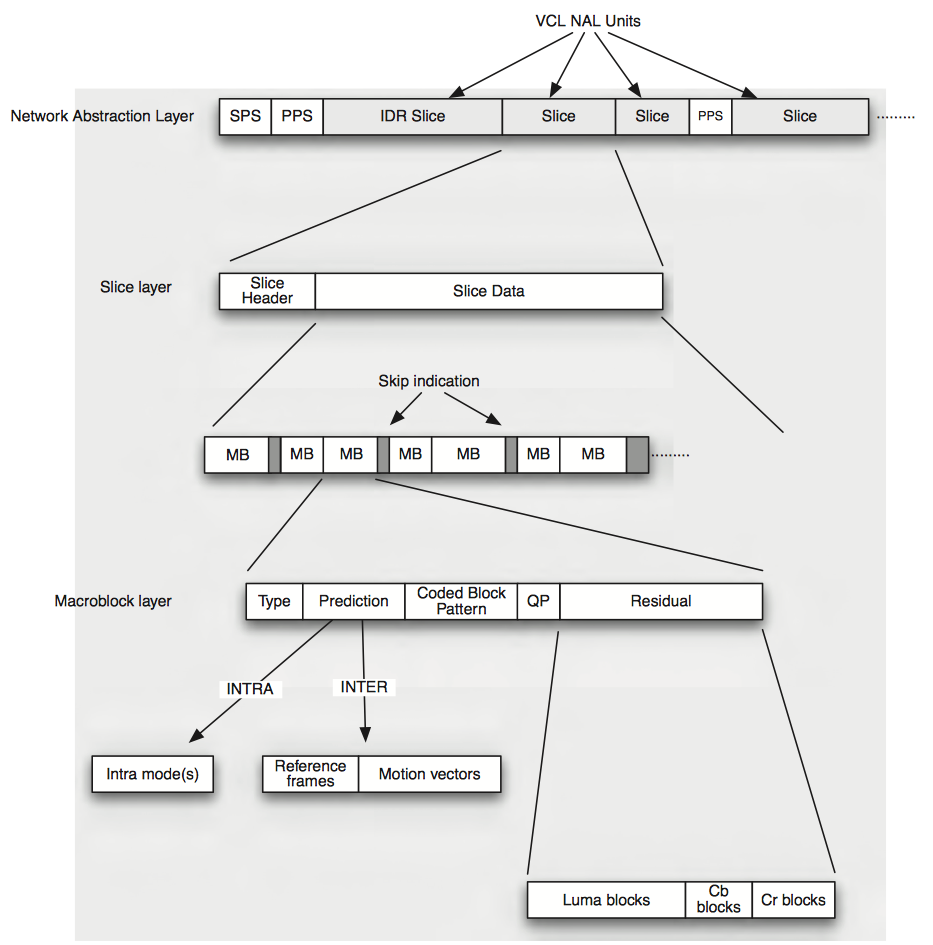
\includegraphics[height=7cm]{syntax.png}
\end{tabular}
\end{center}
\caption[syntax] 
{ \label{fig:syntax} H.264 bitstream syntax}
\end{figure} 

The project is implemented mainly in object oriented paradigm.
Primary concepts of H.264 are abstracted as objects.
A simplified Unified Modeling Language(UML) diagram of the software architecture is shown as below:

\begin{figure} [ht]
\begin{center}
\begin{tabular}{c} %% tabular useful for creating an array of images 
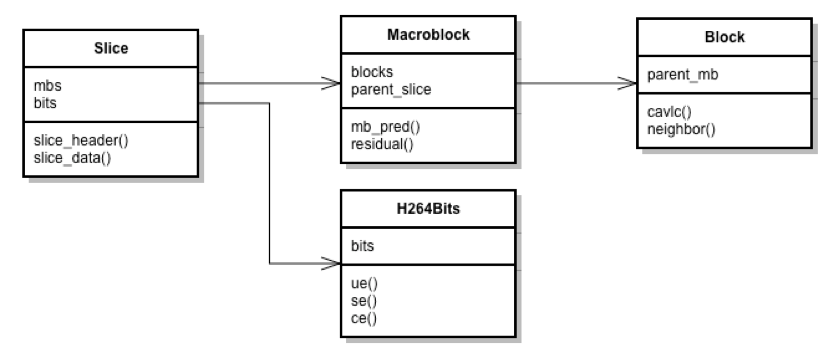
\includegraphics[height=5cm]{uml.png}
\end{tabular}
\end{center}
\caption[uml] 
{ \label{fig:uml} Software architecture UML diagram}
\end{figure} 

The functionalities of these objects are described here.

\subsection{H264Bits}
H264Bits object stores raw bitstream data and entropy decoding methods.
Each slice object contains a reference to the singleton H264Bits object, 
so the binary data can be decoded and transfered to its associated object.

% \begin{verbatim}
%     def u(self,n) # read n bits as a unsigned integer
%     def f(self,n) # read n bits as a signed integer
%     def ue(self) # read bits with variable lenght as unsigned exponential Golomb code
%     def se(self) # read bits with variable lenght as signed exponential Golomb code
%     def ce_coeff_token(self, nC) # decode CAVLC coefficient token with nC
%     def ce_total_zeros(self, tzVlcIndex, maxNumCoeff) # decode number of zeros in coefficients levels
% \end{verbatim}

\subsection{SPS}
SPS object contains sequence parameter set related parsing logic and result.
The parsing methods read parameters from bitstream and store the results as instance variables of the object.
So that these parameters can be shared later. 
There's usually only one SPS object in a sequence.

\subsection{PPS}
PPS object contains picture parameter set related parsing logic and result.
This object has behavior similar to SPS except that there can be multiple PPS objects in a sequence.

\subsection{Slice}
Slice object contains slice header parsing logic, slice related parameters and macroblock objects.
Slice-related paramters from slice header segments are parsed and stored here.
Arbitrary Macroblock objects are contained in this object which is identical to H.264's layer logic.

\subsection{Macroblock}
Macroblock object contains macroblock parsing logic and Luma/Chroma block objects
Macroblock-related parameters are decoded and CAVLC entropy decoding process is invoked here.
The entropy decoded results are stored as Block objects inside this object.

\subsection{Block}
Block object contains Luma/Chroma block's transform coefficients and related decoding methods.
The object also has block id related information stored in it.

\bigskip

Each object also contains its parent object pointer to share data between each other.
So accessing sequence parameter set from a luma block object can be done like this:

\begin{verbatim}
    one_luma_block.mb.slice.sps.some_parameter
\end{verbatim}

There are another two modules for Intra frame decoding: idct and intra\_pred.
These modules are collections of functions for inverse DCT (and dequantization) and intra prediction.

\subsection{IDCT}
This module contains amount of functions to perform dequantization and inverse DCT on block coefficients levels.
Related argument tables are also stored here as module attributes.

\subsection{Intra Prediction}
This module contains amount of functions to generate intra prediction for blocks.

\end{document}